\documentclass[a4paper, 12pt, oneside]{book}
\usepackage{graphicx}
\usepackage[french]{babel}
\usepackage[utf8]{inputenc}
\usepackage[T1]{fontenc}
\frenchbsetup{StandardLists=true}
\usepackage{enumitem}
\usepackage{multirow}
\usepackage{listings}
\usepackage{float}
\usepackage{hyperref}
\usepackage{url}
\usepackage[french]{algorithm}
\usepackage{style/myalgorithm}
\usepackage{amsmath,amsfonts,amssymb}
\newcommand{\fBm}{\emph{fBm}~}
\newcommand{\etal}{\emph{et al.}~}
\newcommand{\glAd}{\emph{GL4D}~}
\newcommand{\apiopengl}{API OpenGL\textsuperscript{\textregistered}~}
\newcommand{\opengl}{OpenGL\textsuperscript{\textregistered}~}
\newcommand{\opengles}{OpenGL\textsuperscript{\textregistered}ES~}
\newcommand{\clang}{langage \texttt{C}}
\newcommand{\codesource}{\textsc{Code source}~}
\floatstyle{ruled}
\newfloat{programslist}{htbp}{locs}
\newcommand{\listofprograms}{\listof{programslist}{Liste des codes source}}
\newcounter{program}[subsection]
\renewcommand{\theprogram}{\arabic{chapter}.\arabic{program}}

\newenvironment{program}[1]{
  \if\relax\detokenize{#1}\relax
  \gdef\mycaption{\relax}
  \else
  \gdef\mycaption{#1}
  \fi
  \refstepcounter{program}
  \addcontentsline{locs}{section}{#1}
  \footnotesize
}{
  \begin{description}
    \item[\codesource \theprogram]--~\mycaption
  \end{description}
}

\begin{document}
\begin{titlepage}
  \begin{center}
    \begin{tabular*}{\textwidth}{l@{\extracolsep{\fill}}r}
      
\includegraphics[height=1.5cm]{images/m1info.png}&
      
\includegraphics[height=1.5cm]{images/oaccueil.png}
    \end{tabular*}
    \small 
    \rule{\textwidth}{.5pt}~\\
    \large 
    \textsc{Université Paris 8 - Vincennes à Saint-Denis}\vspace{0.5cm}\\
    \textbf{M1 MIASHS : Big Data et fouille de données}\vspace{3.0cm}\\
    \Large
    \textbf{TP: Application Dataiku}\vspace{1.5cm}\\
    \large
    \textbf{PANCHALINGAMOORTHY \textsc{Gajenthran}}\vspace{1.5cm}\\
  \end{center}\vspace{1.5cm}~\\
  \begin{tabular}{ll}
    \hspace{-0.45cm}Organisme d'accueil~:~&~Université Paris 8\\
    \hspace{-0.45cm}Cours ~:~&~Visualisation de masses de données\\
  \end{tabular}
\end{titlepage}
\frontmatter

%% Table des matières
\tableofcontents
\mainmatter

%% Introduction
\chapter[Introduction]{Introduction}

  \begin{figure}[H]
    \centering
    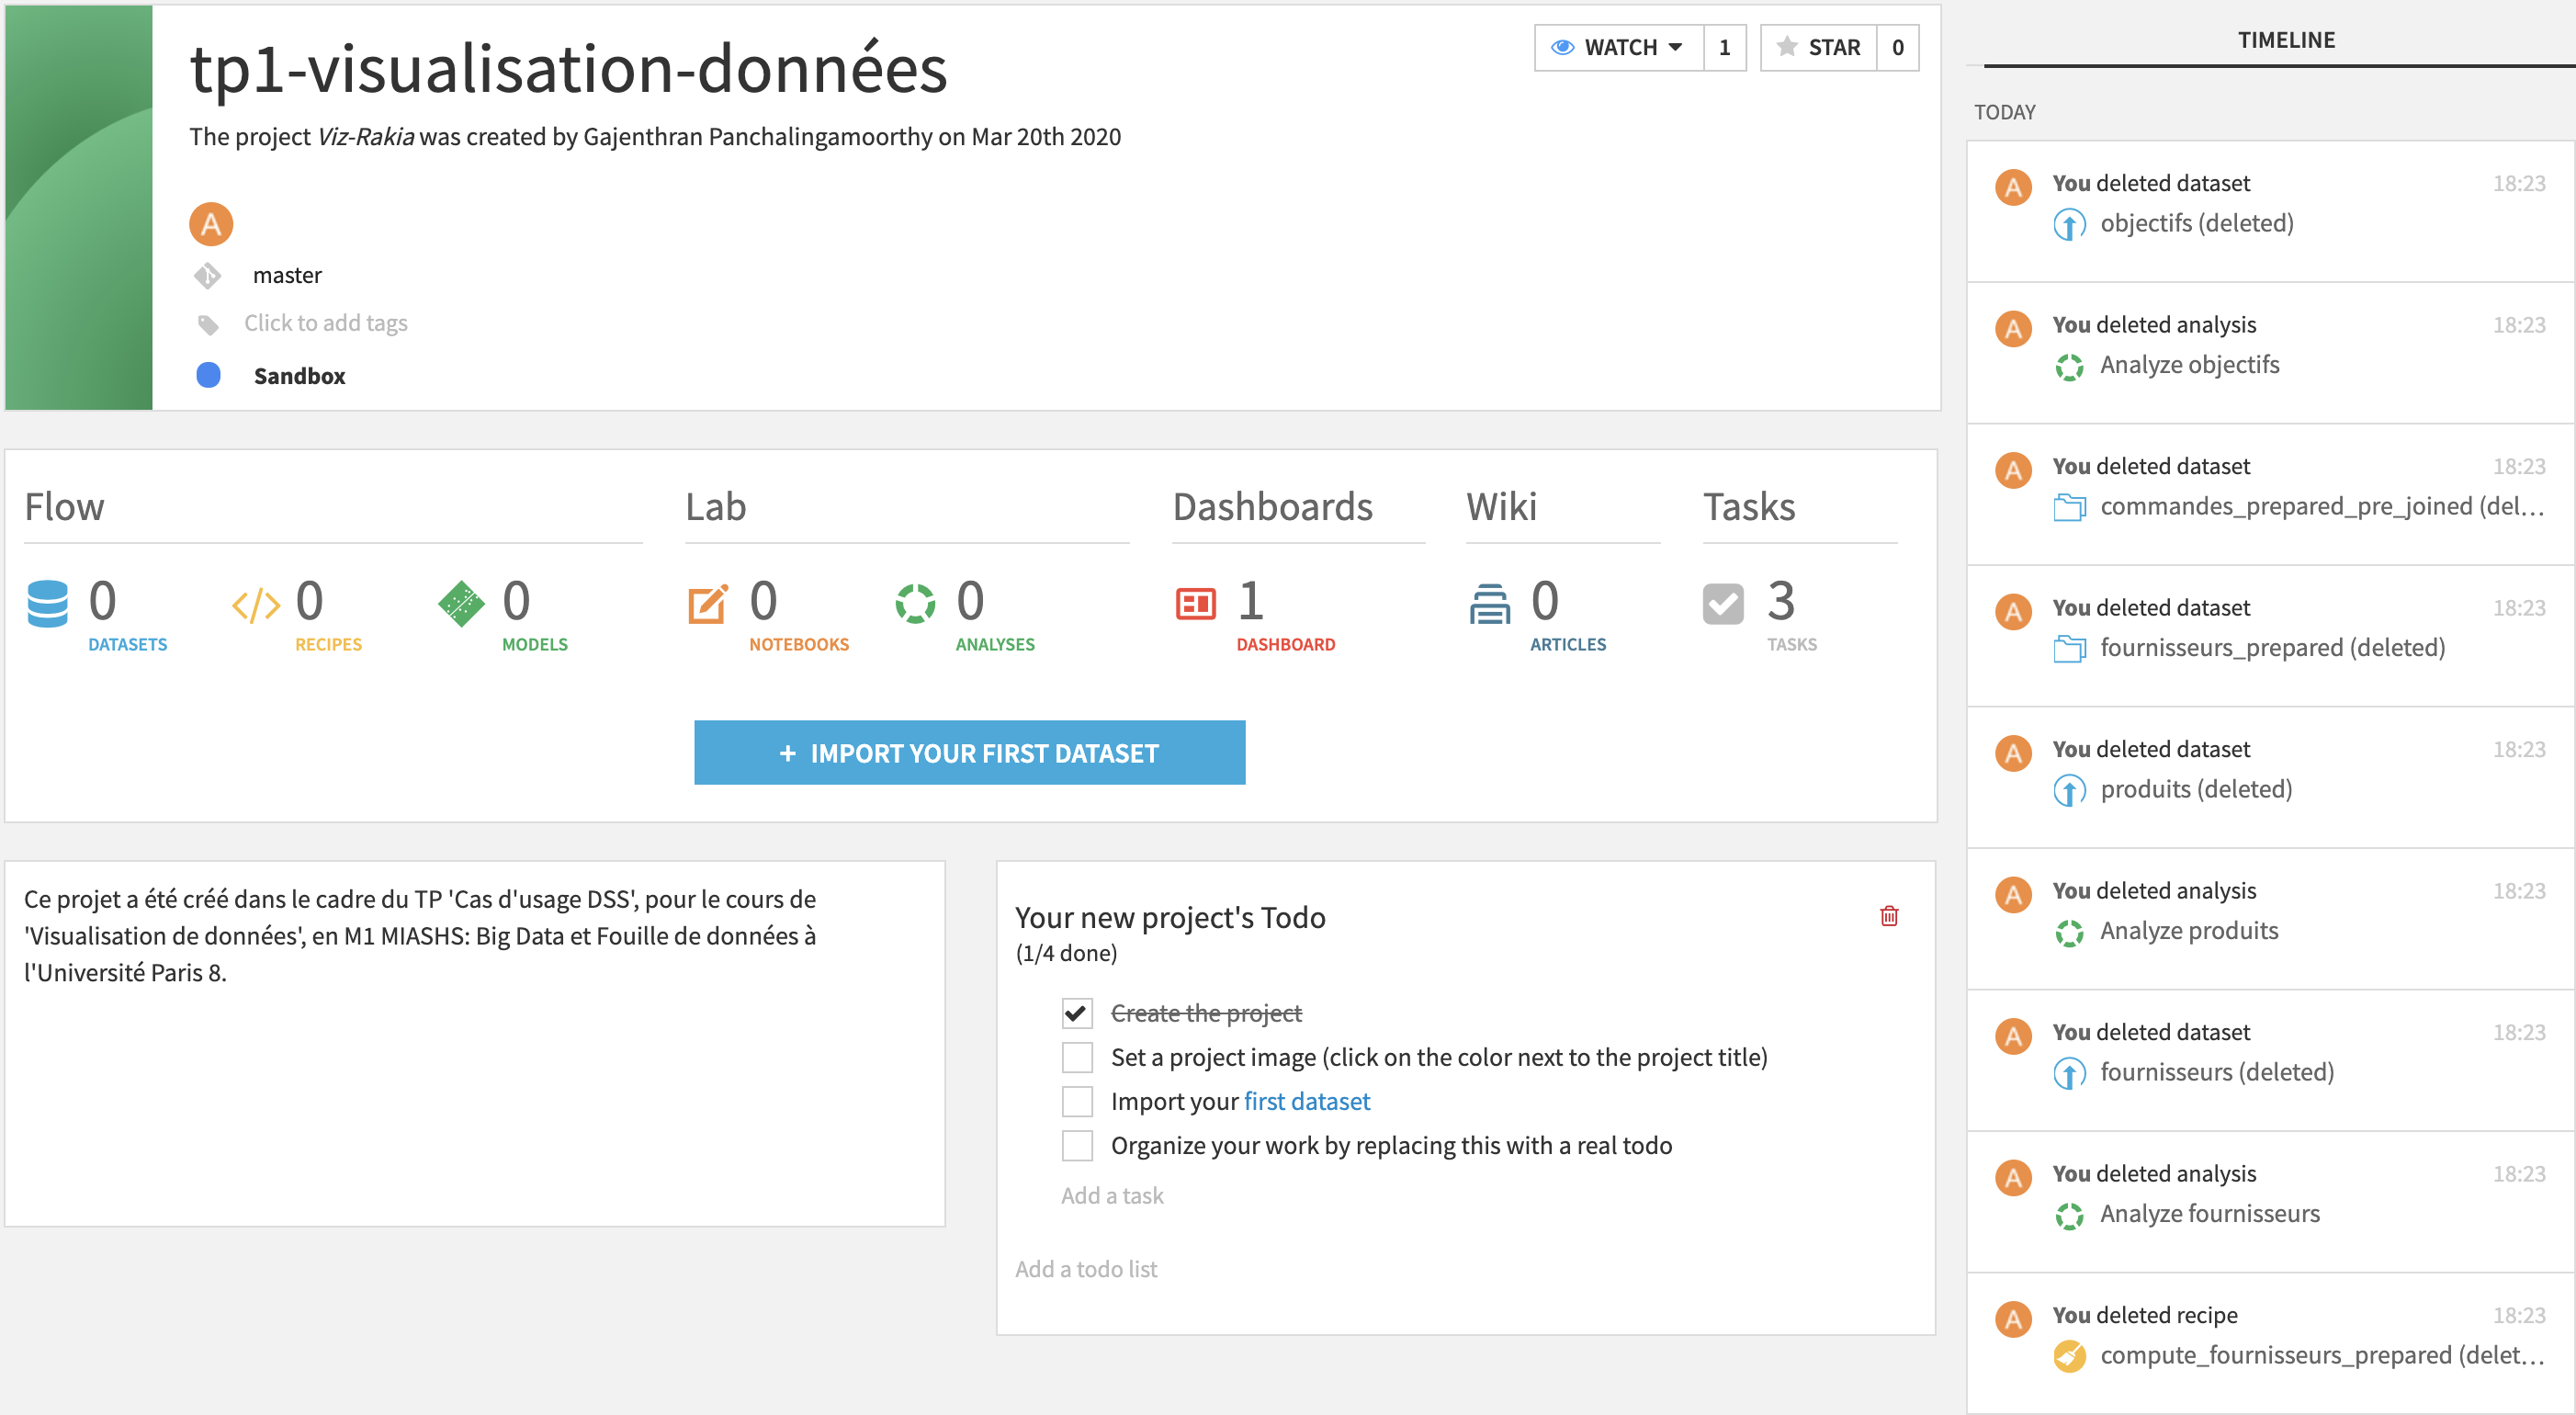
\includegraphics[width=0.7\textwidth]{images/intro-home}
    \caption{Projet \textit{tp1-visualisation-données}}
    \label{fig:intro-home}
  \end{figure}

\chapter{Développement} 
\begin{itemize}
  \item Texte en \texttt{gras}
  \item Texte en \textit{italique}
  \item Référence à une image \ref{fig:intro-home}
  \item Citer un auteur \cite{tourism}
\end{itemize}

\chapter{Conclusion}

\bibliographystyle{alpha}
\bibliography{memoire}
\end{document}
